%!TEX TS-program = xelatex
\documentclass[]{friggeri-cv}
\usepackage{afterpage}
\usepackage{hyperref}
\usepackage{color}
\usepackage{xcolor}
\usepackage{xeCJK}
\setCJKmainfont[BoldFont={Microsoft JhengHei Bold}]{Microsoft JhengHei}
\setCJKmonofont{PMingLiU}
\setCJKsansfont{DFKai-SB}
\newCJKfontfamily[cuhei]\cuti{Microsoft JhengHei Bold}
\hypersetup{
    pdftitle={},
    pdfauthor={},
    pdfsubject={},
    pdfkeywords={},
    colorlinks=false,       % no lik border color
   allbordercolors=white    % white border color for all
}
\addbibresource{bibliography.bib}
\RequirePackage{xcolor}
\definecolor{pblue}{HTML}{0395DE}

\begin{document}
\header{于}{润泽}
      {北京师范大学,理科试验班}
      
% Fake text to add separator      
\fcolorbox{white}{gray}{\parbox{\dimexpr\textwidth-2\fboxsep-2\fboxrule}{%
.....
}}

% In the aside, each new line forces a line break
\begin{aside}
\section{\cuti 生日}
1994.11.18
\section{\cuti 性别}
男
\section{\cuti 民族}
汉
\section{\cuti 籍贯}
河北唐山
\section{\cuti 政治面貌}
共青团员
\section{\cuti 地址}
海淀区~新街口外大街19号~北京师范大学
\section{\cuti 电话}
+86~188~1147~7848
\section{Mail}
\href{mailto:yurunze@mail.bnu.edu.cn}{\textbf{yurunze@}\\mail.bnu.edu.cn}
\href{mailto:watrz@hotmail.com}{\textbf{watrz@}\\hotmail.com}
\section{\cuti 计算机技能}
    ~
    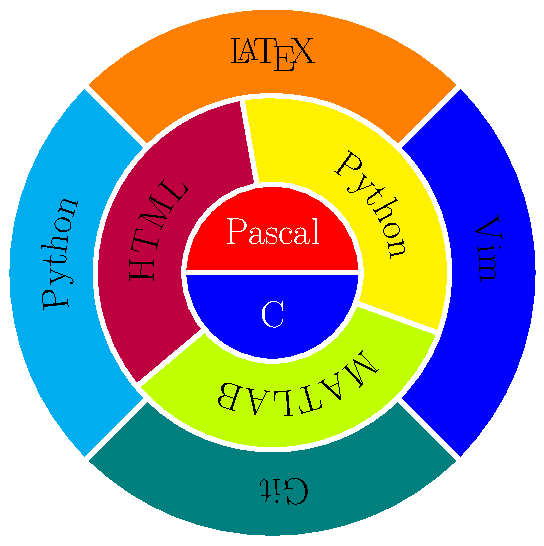
\includegraphics[scale=0.42]{img/programming.pdf}
    ~
  \section{\cuti 操作系统}
    \textbf{Windows}
\includegraphics[scale=0.16]{img/5stars}
    \textbf{GNU/Linux}
\includegraphics[scale=0.16]{img/4stars}
  \section{\cuti 语言}
    \textbf{English}
\includegraphics[scale=0.16]{img/5stars}
    \textbf{Deutsch}
\includegraphics[scale=0.16]{img/3stars}
    \textbf{日本語}
\includegraphics[scale=0.16]{img/2stars}
\end{aside}
\section{\cuti 目标岗位}
技术文案专员(实习生)
\section{\cuti 项目经历}
\begin{entrylist}
  \entry
    {2013 - 2015}
    {\cuti 项目名称}
    {项目支持类型}
    {项目主要研究内容\\}
\end{entrylist}

\section{\cuti 教育经历}
\begin{entrylist}
  \entry
    {2012 - 2016}
    {\cuti 物理学 学士学位}
    {北京师范大学理科试验班(在读)}
    {研究方向:计算物理,微磁学\\
    参与竞赛:xxxxxxxxx\\
    骨干经历:xxxxxxxxx\\}
\end{entrylist}

\section{\cuti 荣誉~\&奖励}
\begin{entrylist}
  \entry
    {09/2014}
    {\cuti 论文名称,作者}
    {论文发布单位}
    {\emph{论文大概内容}}
\end{entrylist}\\

\section{\cuti 课余活动}
\begin{entrylist}
\entry{2014 - 今}{\cuti 北京诗词学会}{会员}{创作并发表了一些近体诗和词}
\entry{2012 - 今}{\cuti 骑行}{}{累计骑行两万余公里,旅程涉及河北、北京、天津、山东、山西、河南和台湾}
\end{entrylist}

\vspace{40pt}

\begin{flushright}
\emph{二〇一五年四月二日}
\end{flushright}
\begin{flushright}
\emph{于润泽}
\end{flushright}

%%% This piece of code has been commented by Karol Kozioł due to biblatex errors. 
% 
%\printbibsection{article}{article in peer-reviewed journal}
%\begin{refsection}
%  \nocite{*}
%  \printbibliography[sorting=chronological, type=inproceedings, title={international peer-reviewed conferences/proceedings}, notkeyword={france}, heading=subbibliography]
%\end{refsection}
%\begin{refsection}
%  \nocite{*}
%  \printbibliography[sorting=chronological, type=inproceedings, title={local peer-reviewed conferences/proceedings}, keyword={france}, heading=subbibliography]
%\end{refsection}
%\printbibsection{misc}{other publications}
%\printbibsection{report}{research reports}

\end{document}
